\documentclass[11pt, oneside]{article}   	% use "amsart" instead of "article" for AMSLaTeX format
\usepackage{geometry}                		% See geometry.pdf to learn the layout options. There are lots.
\geometry{letterpaper}                   		% ... or a4paper or a5paper or ... 
%\geometry{landscape}                		% Activate for for rotated page geometry
%\usepackage[parfill]{parskip}    		% Activate to begin paragraphs with an empty line rather than an indent
\usepackage{graphicx}				% Use pdf, png, jpg, or eps� with pdflatex; use eps in DVI mode
								% TeX will automatically convert eps --> pdf in pdflatex		
\usepackage{amssymb}
\usepackage{amsmath}
\graphicspath{{/Users/telliott_admin/Dropbox/Tex/png/}}
\usepackage{parskip}

\title{Injection, surjection and inverse sine}
%\author{The Author}
\date{}							% Activate to display a given date or no date

\begin{document}
\maketitle
%\section{}
%\subsection{}
\noindent
\large
The question of whether a function has a reverse (is reversible) comes up naturally in the study of techniques of integration.  Consider this triangle
\begin{center}
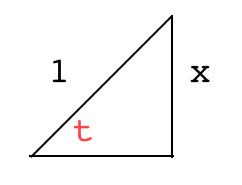
\includegraphics [scale=0.5] {arcsin4.png}
\end{center}
We have constructed the triangle so that the sine of the angle $t$ is equal to $x/1$:
\[ \sin t = x \]
The reverse of sine is the function $\arcsin$ (or $\sin^{-1}$):
\[ \sin^{-1} x = t \]
Read this as:  arcsine (inverse sine) of $x$ is equal to $t$.  Alternatively, we can say that $t$ is the angle whose sine is equal to $x$.  It doesn't really matter that there is no technique for computation other than trying different values for $x$, calculating $\sin x$, and comparing that with the $t$ we are given.

Now, by the Pythagorean Theorem, the third side of the triangle has length $\sqrt{1-x^2}$, and in terms of angle $t$, we have that
\[ \cos t = \sqrt{1-x^2} \]
This becomes useful where we have an integral like:
\[ \int \frac{1}{\sqrt{1-x^2}} \ dx \]
We cannot just substitute for $1-x^2$ because we don't have the derivative (we don't have an $x$ on top).  But doing a trigonometric substitution, we have that 
\[ \frac{1}{\sqrt{1-x^2}} = \frac{1}{\cos t} \]
To complete the substitution, we need to find $dx$ in terms of $dt$:
\[ x = \sin t \]
\[ dx = \cos t \ dt \]
So that gives:
\[ \int \frac{1}{\cos t} \  \cos t \ dt \]
which simplifies nicely to:
\[ \int dt = t \]
To complete the solution, we need to switch back to the original variable $x$.
\[ t = \sin^{-1} x \]
Thus:
\[ \int \frac{1}{\sqrt{1-x^2}} \ dx = \sin^{-1} x + C \]

It may seem strange at first that this integral in Cartesian coordinates ($xy$-"land") gives a result in terms of the angle $t$, but consider that the equation of the unit circle is
\[ x^2 + y^2 = 1 \]
so
\[ y = + \sqrt{1 - x^2} \]
is the equation of the top half of the circle (above the $x$-axis).  The integral that we have computed is the area under this curve, under the right limits it is the area of the unit circle, so naturally this result involves $\pi$.

Another way to approach this (which involves the same relationships) is to use differentials

\[ x = \sin t \]
\[ dx = \cos t \ dt \]
\[ \frac{dt}{dx} = \frac{1}{\cos t} \]
\[ \frac{d}{dx} t =  \frac{1}{\cos t} \]
\[ \frac{d}{dx} \sin^{-1} x =  \frac{1}{\sqrt{1-x^2}} \]
\[ \int \frac{d}{dx} \sin^{-1} x \ dx = \int \frac{1}{\sqrt{1-x^2}} \ dx \]
\[ \sin^{-1} x =  \int \frac{1}{\sqrt{1-x^2}} \]

In working with reverse functions, we have to consider carefully the domain and range of each. (more)

We also have to consider whether a given function even has an inverse.  Consider (following Koblitz)
\[ f = x^3; \ \ \ g = x^{1/3} \]

For these two functions to qualify as inverses we require that
\[ x = f(g(x)) \]
and
\[ x = g(f(x)) \]

However, this is not true of the square root function 
\[ f = x^2; \ \ \ g = x^{1/2} \]
because there are two real numbers that satisfy $x^2 = 2$ for example, but when we take the square root, we define the positive root as the result of the function $g$.

\subsection*{injective}

In the language of set theory, consider (the set of) all real numbers that are in the domain of $f$---call that set $A$, and then call the corresponding values of $f(x)$ the set $B$.  $B$ is range of $f$.

If and only if each of these numbers yields a \emph{different} value in $B$, then it may be possible to come up with an inverse function $g$ which maps from the range back to the domain.

Such a function is described as \emph{injective}.  On the other hand, if two different values $a_1, a_2$ in the domain of $f$ yield the same value $f(a_1) = f(a_2)$, then the function is non-injective.

Koblitz:

	Let $A$ and $B$ be sets and let $f:  A \rightarrow B$ be a function.  We say that $f$ is injective or one-to-one if $f(x) = f(y)$ implies that $x = y$.  See the wikipedia figure, upper-left panel.
	
\begin{center}
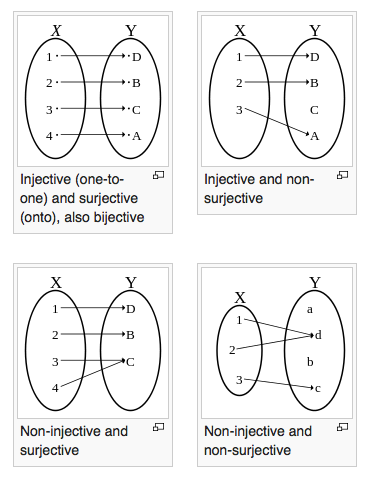
\includegraphics [scale=0.6] {injective.png}
\end{center}

\subsection*{surjective}

Surjective is a statement about the range and co-domain of $f$.  If there numbers in the co-domain that do not correspond to $f(x)$ for \emph{any} $x$ in the range of $f$, then $f$ is not surjective.  See the upper-right panel.

Koblitz:

	We say that $f$ is surjective or onto if for every $b \in B$ there is an $a \in A$ such that $f(a) = b$.
	
	If $f$ is both injective and surjective, then $f$ is bijective or one-to-one and onto.

A simple test is the \textbf{horizontal line test}.  If a horizontal line intersects the graph of $f(x)$ at more than one point, the function is not injective and not reversible.  (Those two points are different values of $x$ which share the same value $y = f(x)$).

The function $f(x) = x^2$ is a parabola and it fails the horizontal line test.  On the other hand, the graph of $f(x) = x^3$ is:

\begin{center}
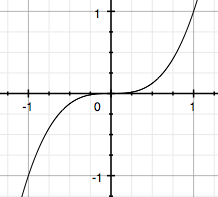
\includegraphics [scale=0.5] {y=x^3.png}
\end{center}

and it passes the test.  (However $x^3 - x^2$ fails).

Let's look at the graph of the arcsin and arccosine functions.

\begin{center}
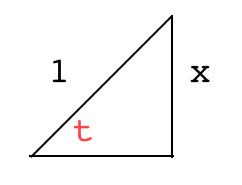
\includegraphics [scale=0.5] {arcsin4.png}
\end{center}

These graphs are simply plots of the more familiar sine and cosine that have been rotated counter-clockwise by 90 degrees, and also flipped left-to-right (to make $x$-values increase to the right, as usual.

By definition, a function assigns a unique value of $y$ for each value of $x$.  Since these functions repeat, we limit the domain appropriately.  For arcsin, the domain is $y = -\pi/2 \rightarrow \pi/2$, while for arccose it is $y = 0 \rightarrow \pi$.

\subsection*{Note on constants}

We looked at the function $1/\sqrt{1-x^2}$, but a more general form is $1/\sqrt{a^2 - x^2}$, for a constant $a$.

There are two ways to deal with this.  The first is to scale the triangle so that the hypotenuse is of length $a$ and the side adjacent to angle $t$ is $\sqrt{a^2 - x^2}$.  Then, we have

\[ x = a \sin t \]
\[ \sqrt{a^2 - x^2} = a \cos t \]
\[ dx = a \cos t \ dt \]
\[ \int \frac{1}{\sqrt{a^2 - x^2}} \ dx = \int \frac{1}{a \cos t} a \cos t \ dt  = t \]
\[ t = \sin^{-1} \frac{x}{a} \]

Another way to do this is to manipulate the original equation:

\[ \int \frac{1}{\sqrt{a^2 - x^2}} \ dx \]
\[ = \int \frac{1}{a \sqrt{1 - x^2/a^2}} \ dx \]
\[ = \frac{1}{a} \int \frac{1}{\sqrt{1 - x^2/a^2}} \ dx \]
Now let $u = x/a$  so that $a \ du = dx$ and then
\[ = a \ \frac{1}{a} \int \frac{1}{\sqrt{1 - u^2}} \ du \]
\[ =  \int \frac{1}{\sqrt{1 - u^2}} \ du \]
We obtain 
\[ t = \sin^{-1} u \]
\[ = \sin^{-1} \frac{x}{a} \]
as before.

\end{document}  